%%%%%%%%%%%%%%%%%%%%%%%%%%%%%%%%%%%%%%%%%%%%%%%%%%%%%%%%%%%%%%%%
%%%%%%%%%%%%%%%%%%%%%%%%%%%%%%%%%%%%%%%%%%%%%%%%%%%%%%%%%%%%%%%%
%%%%
%%%% This text file is part of the source of 
%%%% `Introduction to High-Performance Scientific Computing'
%%%% by Victor Eijkhout, copyright 2012
%%%%
%%%% This book is distributed under a Creative Commons Attribution 3.0
%%%% Unported (CC BY 3.0) license and made possible by funding from
%%%% The Saylor Foundation \url{http://www.saylor.org}.
%%%%
%%%%
%%%%%%%%%%%%%%%%%%%%%%%%%%%%%%%%%%%%%%%%%%%%%%%%%%%%%%%%%%%%%%%%
%%%%%%%%%%%%%%%%%%%%%%%%%%%%%%%%%%%%%%%%%%%%%%%%%%%%%%%%%%%%%%%%

In much of this chapter, we assumed that a problem could be perfectly
divided over processors, that is, a processor would always be
performing useful work, and only be \indexterm{idle}
because of latency in communication. In practice, however, a processor
may be idle because it is waiting for a message, and the sending
processor has not even reached the send instruction in its code. Such
a situation, where one processor is working and another is idle, is
described as \indextermbus{load}{unbalance}: there is no intrinsic reason
for the one processor to be idle, and it could have been working if we
had distributed the work load differently.

There is an asymmetry between processors having too much work and
having not enough work: it is better to have one processor that
finishes a task early, than having one that is overloaded so that all
others wait for it.

\begin{exercise}
  Make this notion precise. Suppose a parallel task takes time~1 on
  all processors but one. 
  \begin{itemize}
  \item Let $0<\alpha<1$ and let one processor take time
    $1+\alpha$. What is the speedup and efficiency as function of the
    number of processors? Consider this both in the Amdahl and
    Gustafsson sense (section~\ref{sec:amdahl}).
  \item Answer the same questions if one processor takes time $1-\alpha$.
  \end{itemize}
\end{exercise}

Load balancing is often expensive since it requires moving relatively
large amounts of data. For instance, section~\ref{sec:pspmvp} has an
analysis showing that the data exchanges during a sparse matrix-vector
product is of a lower order than what is stored on the
processor. However, we will not go into the actual cost of moving: our
main concerns here are to balance the workload, and to preserve any
locality in the original load distribution.

\Level 2 {Load balancing of independent tasks}

Let us first consider the case of a job that can be partitioned into
independent tasks that do not communicate. An example would be
computing the pixels of a \indexterm{Mandelbrot set} picture, where
each pixel is set according to a mathematical function that does not
depend on surrounding pixels. If we could predict the time it would
take to draw an arbitrary part of the picture, we could make a perfect
division of the work and assign it to the processors. This is known as
\emph{static load balancing}\index{load!balancing,static}.

More realistically, we can not predict the running time of a part of
the job perfectly, and we use an \indexterm{overdecomposition} of the
work: we divide the work in more tasks than there are
processors. These tasks are then assigned to a \indexterm{work pool},
and processors take the next job from the pool whenever they finish a
job. This is known as \emph{dynamic load
  balancing}\index{load!balancing, dynamic}. Many graph and
combinatorial problems can be approached this way; see
section~\ref{sec:task-parallel}. For task assignment in a multicore
context, see section~\ref{sec:multicore-block}.

There are results that show that randomized assignment of tasks to
processors is statistically close to optimal~\cite{KarpZhang88}, but
this ignores the aspect that in scientific computing tasks typically
communicate frequently.

\Level 2 {Load balancing as graph problem}
\label{sec:graph-loadbalancing}

Next let us consider a parallel job where the parts do communicate. In
this case we need to balance both the scalar workload and the
communication.

A parallel computation can be formulated as a graph (see
Appendix~\ref{app:graph} for an introduction to graph theory) where the
processors are the vertices, and there is an edge between two vertices
if their processors need to communicate at some point. Such a graph is
often derived from an underlying graph of the problem being solved.
As an example consider the matrix-vector product $y=Ax$ where
$A$~is a sparse matrix, and look in detail at the processor that is
computing~$y_i$ for some~$i$. The statement $y_i\leftarrow y_i+A_{ij}x_j$
implies that this processor will need the value~$x_j$, so, if this
variable is on a different processor, it needs to be sent over.

We can formalize this: Let the vectors $x$ and~$y$ be distributed
disjointly over the processors, and define uniquely $P(i)$ as the
processor that owns index~$i$. Then there is an edge $(P,Q)$ if there
is a nonzero element~$a_{ij}$ with $P=P(i)$ and $Q=P(j)$. This graph
is undirected if the matrix is \indexterm{structurally symmetric},
that is $a_{ij}\not=0\Leftrightarrow a_{ji}\not=0$.

The distribution of indices over the processors now gives us vertex
and edge weights: a processor has a vertex weight that is the number
of indices owned by it; an edge $(P,Q)$ has a weight that is the number of
vector components that need to be sent from~$Q$ to~$P$, as described above.

The load balancing problem can now be formulated as
follows:
\begin{quote}
  Find a partitioning $\bbP=\cup_i \bbP_i$, such the variation in
  vertex weights is minimal, and simultaneously the edge weights are
  as low as possible.
\end{quote}
Minimizing the variety in vertex weights implies that all processor
have approximately the same amount of work. Keeping the edge weights
low means that the amount of communication is low. These two
objectives need not be satisfiable at the same time: some trade-off is
likely. 

\begin{exercise}
  Consider the limit case where processors are infinitely fast and
  bandwidth between processors is also unlimited. What is the sole
  remaining factor determining the runtime? What graph problem do you
  need to solve now to find the optimal load balance? What property of
  a sparse matrix gives the worst case behaviour?
\end{exercise}

An interesting approach to load balancing comes from spectral graph
theory (section~\ref{app:fiedler}): if $A_G$ is the adjacency matrix
of an undirected graph and $D_G-A_G$ the \indextermbus{graph}{Laplacian},
then the eigenvector~$u_1$ to the smallest eigenvalue zero is
positive, and the eigenvector $u_2$ to the next eigenvalue is
orthogonal to it. Therefore $u_2$ has to have elements of alternating
sign; further analysis shows that the elements with positive sign are
connected, as are the negative ones. This leads to a natural bisection
of the graph.

\Level 2 {Load redistributing}

In certain applications an initial load distribution is clear, but
later adjustments are needed. A~typical example is in \ac{FEM} codes,
where load can be distributed by a partitioning of the physical
domain; see section~\ref{sec:par-spmvp}. If later the discretization
of the domain changes, the load has to be
\emph{rebalanced}\index{load!rebalancing} or
\emph{redistributed}\index{load!redistributing}. In the next
subsection we will see one technique for load balancing and
rebalancing that is aimed at preserving locality.

\Level 2 {Load balancing with space-filling curves}
\label{sec:space-filling}
\index{space-filling curve|(}

In the previous sections we considered two aspects of load balancing:
making sure all processors have an approximately equal amount of work,
and letting the distribution reflect the structure of the problem so
that communication is kept within reason. We can phrase the second
point as follows: we try to preserve the locality of the problem when
we distribute it over a parallel machine.

Striving to preserve locality is not obviously the right strategy. In
\ac{BSP} (see section~\ref{sec:bsp}) a statistical argument is made
that \indexterm{random placement} will give a good load balance as
well as balance of communication.

\begin{exercise}
  Consider the assignment of processes to processors, where the
  structure of the problem is such that 
  each processes only communicates with its
  nearest neighbours, and let processors be ordered in a
  two-dimensional grid. If we do the obvious assignment of the process
  grid to the processor grid, there will be no contention. Now write a
  program that assigns processes to random processors, and evaluate
  how much contention there will be.
\end{exercise}

In the previous section you saw how graph partitioning techniques can
help with the second point of preserving problem locality. In this
section you will see a different technique that is attractive both for
the initial load assignment and for subsequent
\indextermbus{load}{rebalancing}. In the latter case, a processor's
work may increase or decrease, necessitating moving some of the load
to a different processor.

For instance, some problems are adaptively
refined\index{refinement!adaptive}\footnote{For a detailed
  discussion see~\cite{Campbell:octree}.}. This is illustrated in
figure~\ref{fig:octree1}.
\begin{figure}[ht]
%  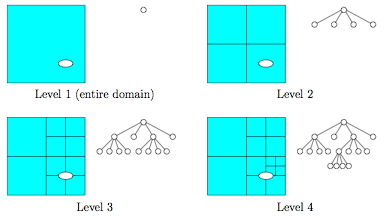
\includegraphics[scale=1]{graphics-public/octree1}
  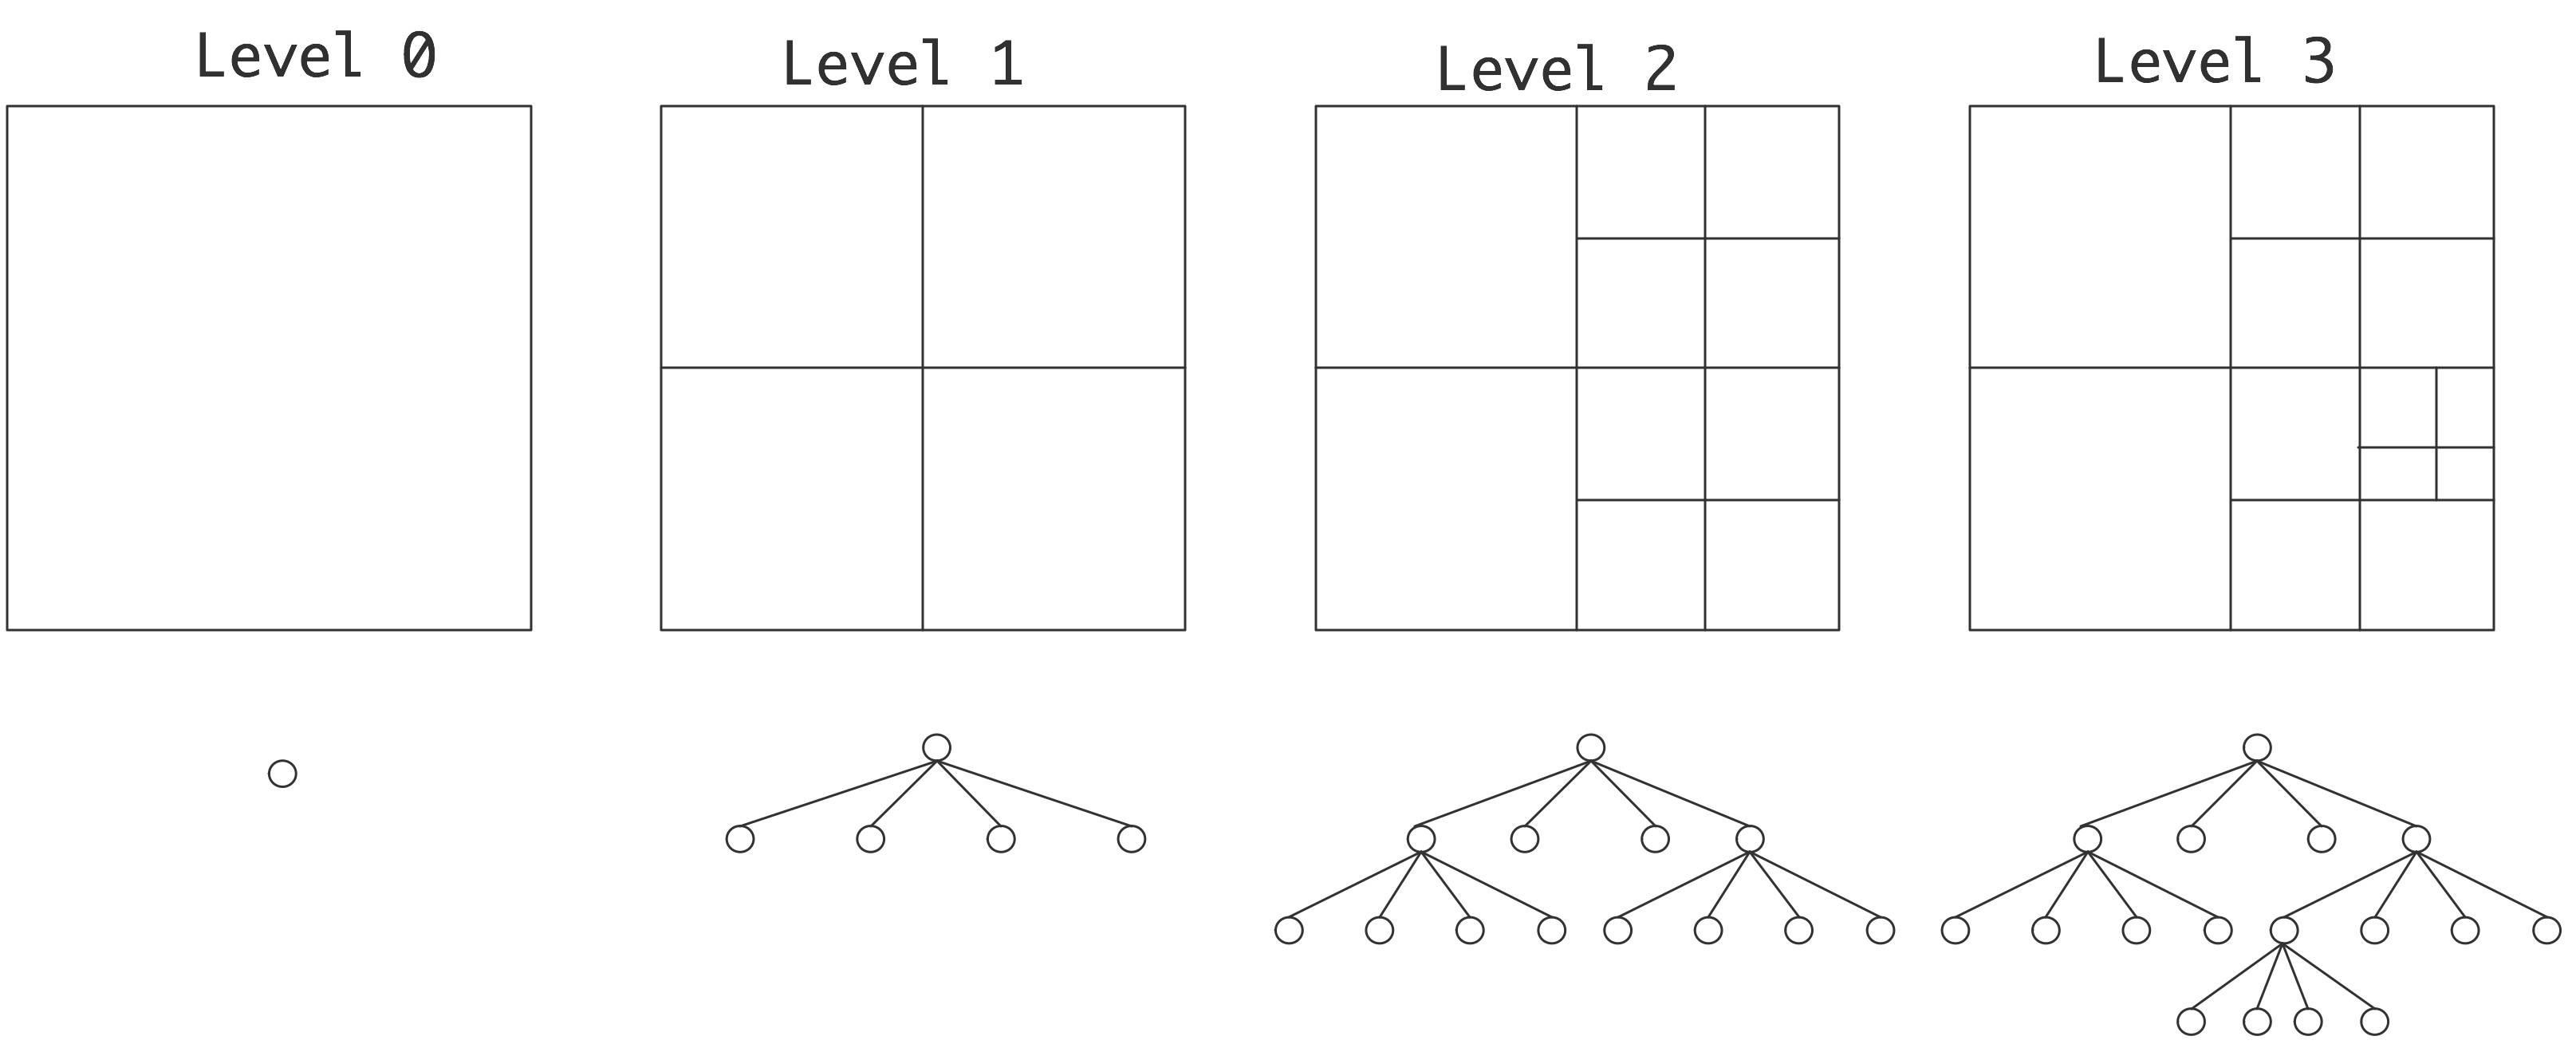
\includegraphics[scale=.14]{graphics-public/my_octree1}
  \caption{Adaptive refinement of a domain in subsquent levels}
  \label{fig:octree1}
\end{figure}
If we keep track of these refinement levels, the problem gets a tree
structure, where the leaves contain all the work.
Load balancing becomes a matter of partitioning the leaves of the
tree over the processors; figure~\ref{fig:octree2}.
\begin{figure}[ht]
%  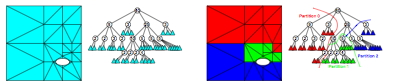
\includegraphics[scale=1]{graphics-public/octree2}
  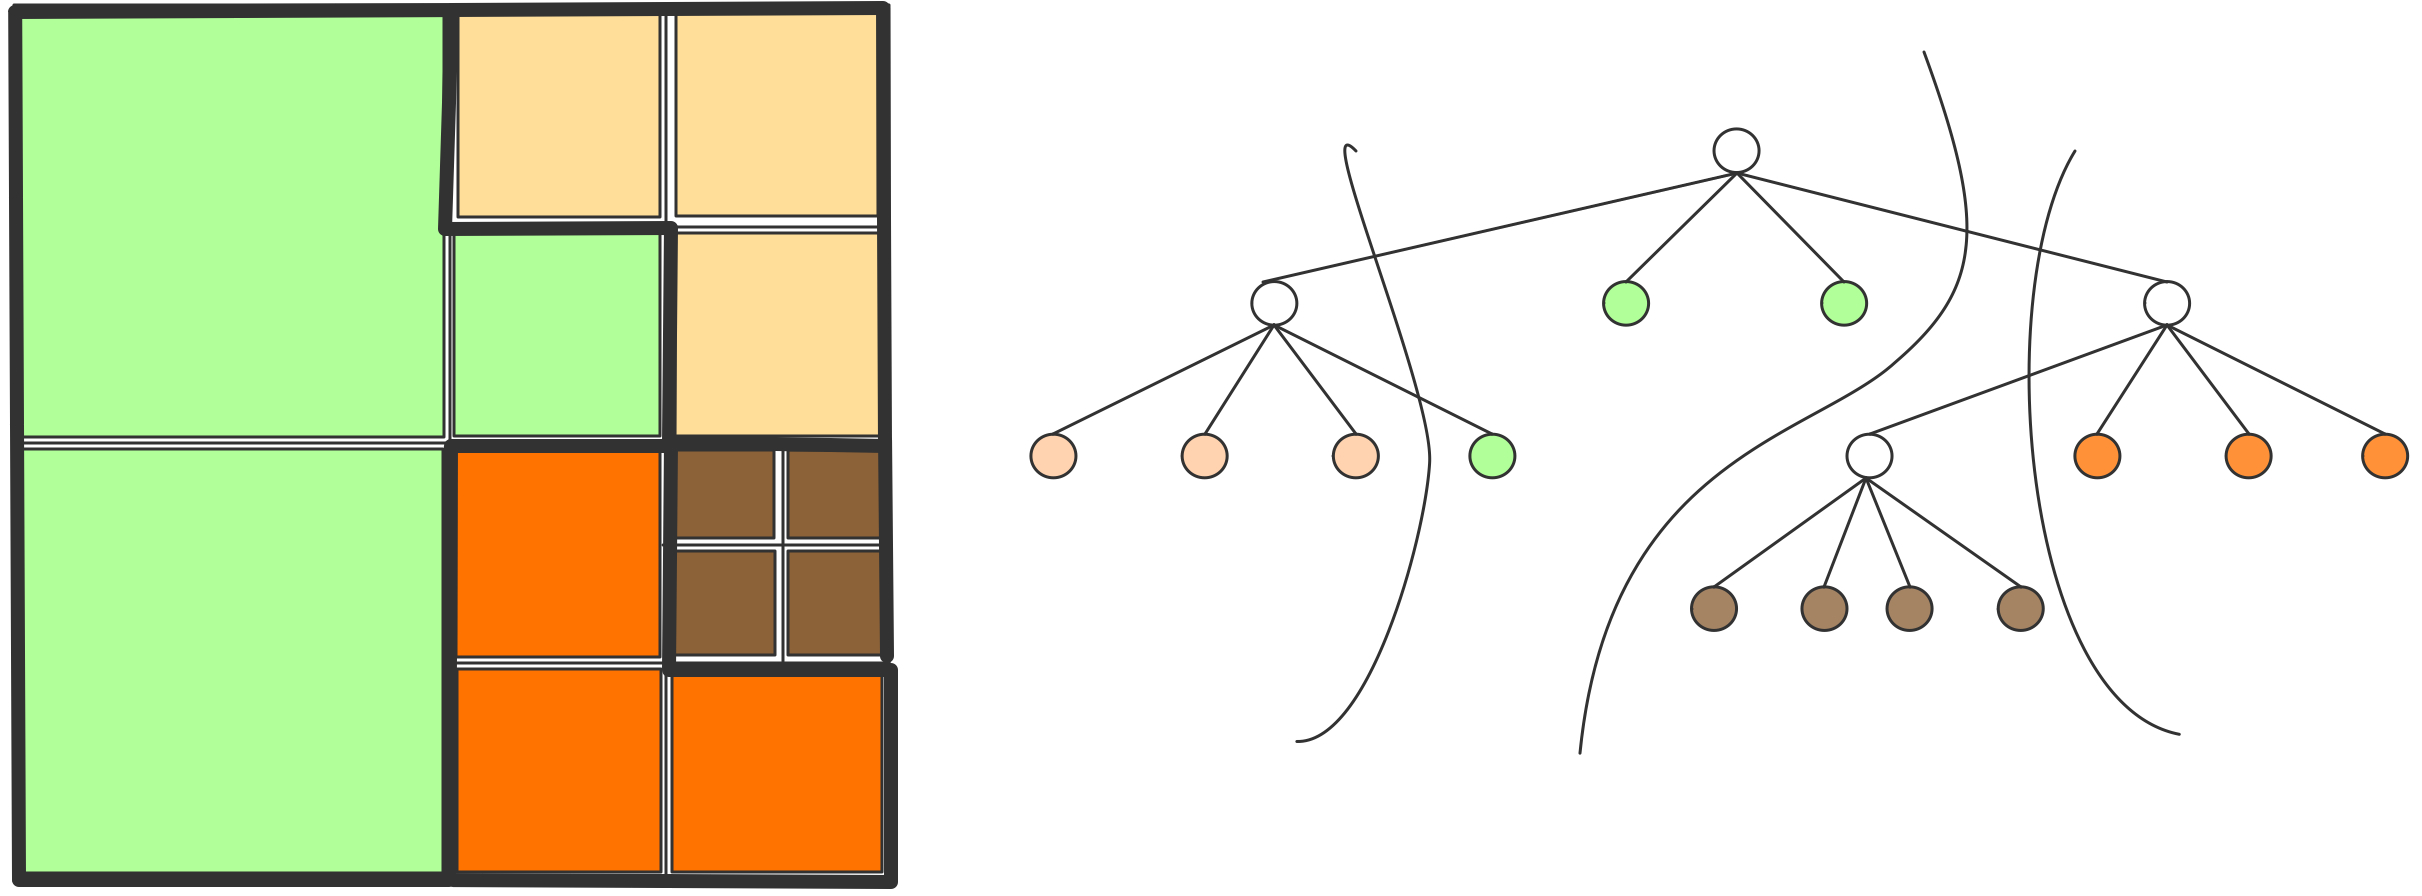
\includegraphics[scale=.18]{graphics-public/my_octree2}
  \caption{Load distribution of an adaptively refined domain}
  \label{fig:octree2}
\end{figure}
Now we observe that the problem has a certain locality: the subtrees
of any non-leaf node are physically close, so there will probably be
communication between them. 
\begin{itemize}
\item Likely there will be more subdomains than processors; to
  minimize communication between processors, we want each processor to
  contain a simply connected group of subdomains. Moreover, we want
  each processor to cover a part of the domain that is `compact' in
  the sense that it has low aspect ratio, and low surface-to-volume
  ratio.
\item When a subdomain gets further subdivided, part of the load of
  its processor may need to be shifted to another processor. This
  process of \indextermbus{load}{redistributing} should preserve
  locality.
\end{itemize}

To fulfill these requirements we use \acfp{SFC}. A \acf{SFC} for the
load balanced tree is shown in figure~\ref{fig:octree-sfc}. We will
not give a formal discussion of \acp{SFC}; instead we
\begin{figure}[ht]
%  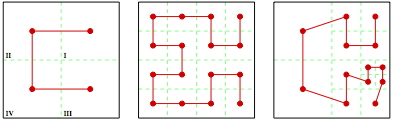
\includegraphics[scale=1]{graphics-public/octree3}
  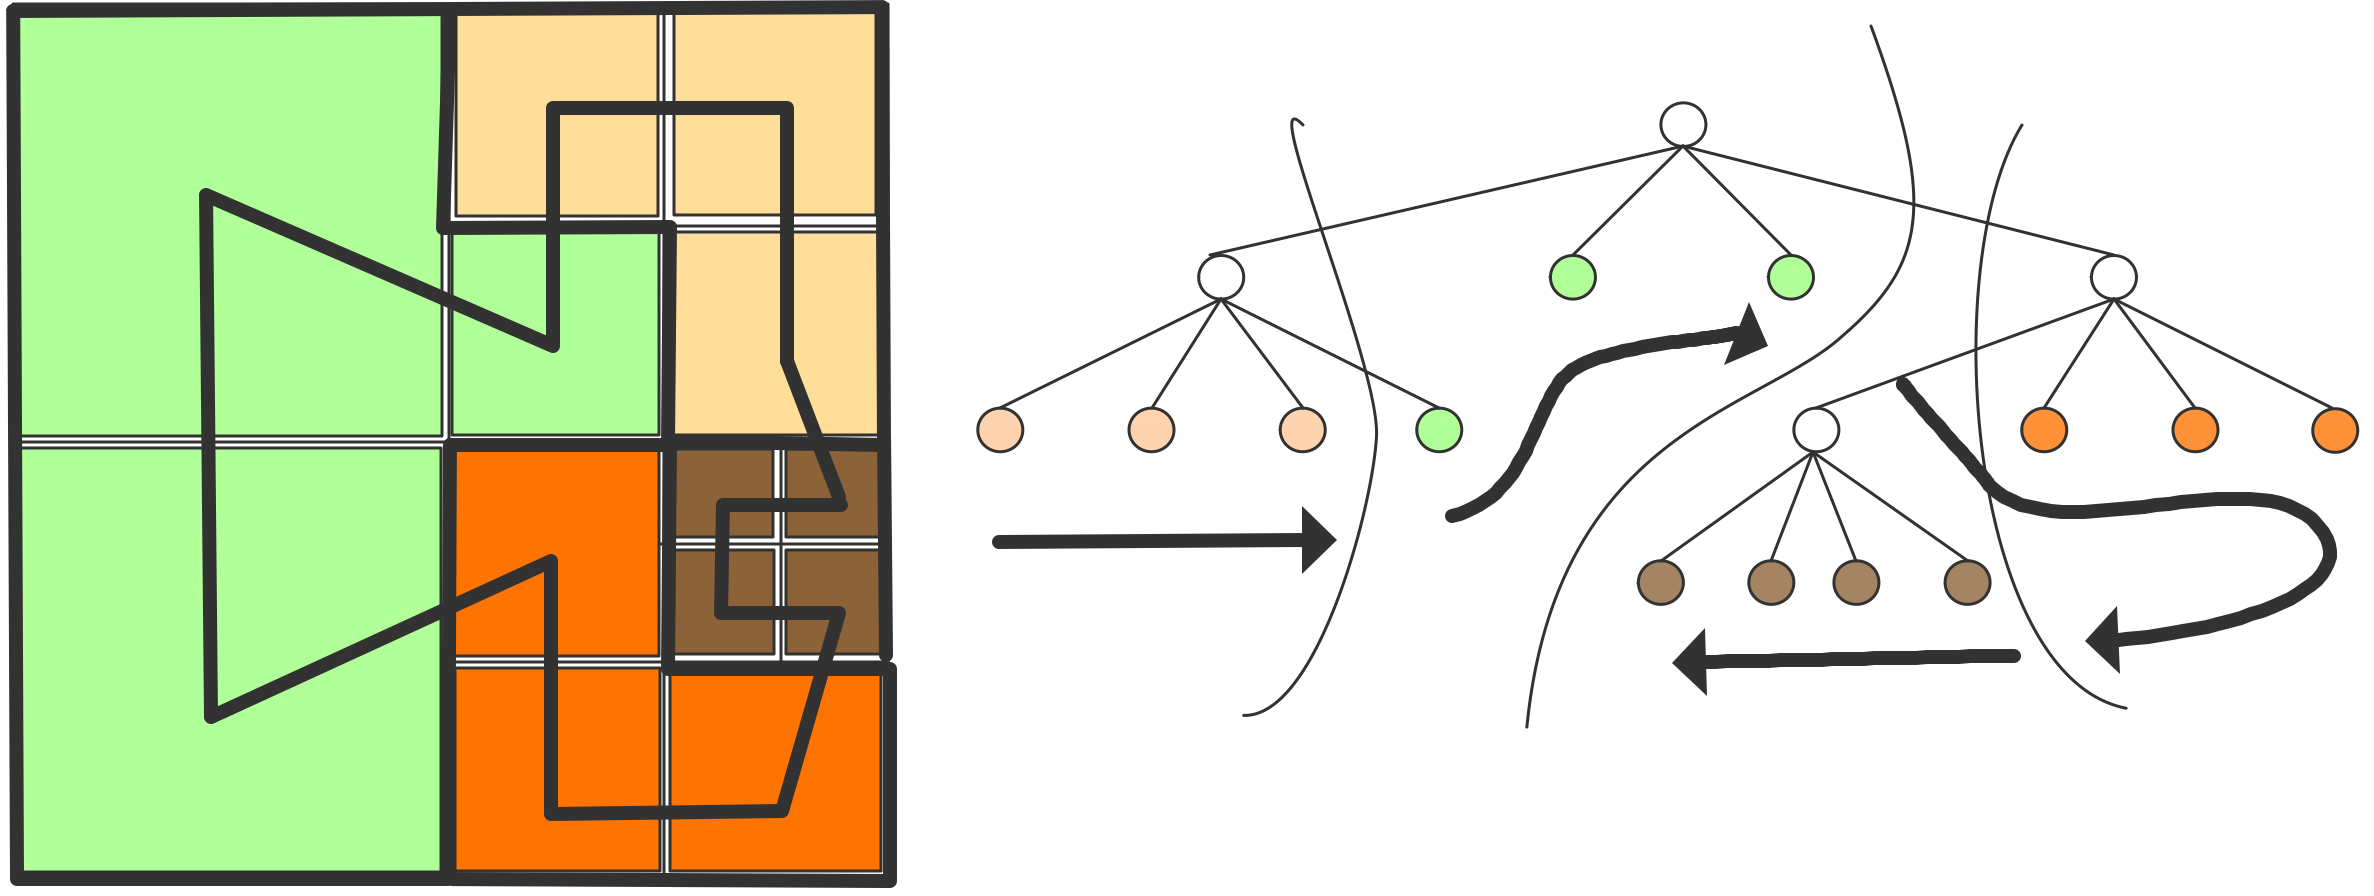
\includegraphics[scale=.18]{graphics-public/my_octree3}
  \caption{A space filling curve for the load balanced tree}
  \label{fig:octree-sfc}
\end{figure}
will let figure~\ref{fig:octree3} stand for a definition: a \ac{SFC} is a
recursively defined curve that touches each subdomain
once\footnote{\acfp{SFC} were introduced by Peano as a mathematical
  device for constructing a continuous surjective function from the
  line segment $[0,1]$ to a higher dimensional cube $[0,1]^d$. This
  upset the intuitive notion of dimension that `you can not stretch
  and fold a line segment to fill up the square'. A~proper treatment
  of the concept of dimension was later given by Brouwer.}.
\begin{figure}[ht]
  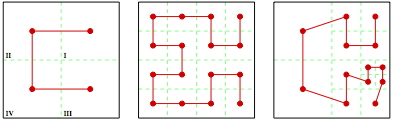
\includegraphics[scale=1]{graphics-public/octree3}
  \caption{Space filling curves, regularly and irregularly refined}
  \label{fig:octree3}
\end{figure}
The \ac{SFC} has the property that domain elements that are close
together physically will be close together on the curve, so if we map
the \ac{SFC} to a linear ordering of processors we will preserve the
locality of the problem. 

More importantly, if the domain is refined by
another level, we can refine the curve accordingly. Load can then be
redistributed to neighbouring processors on the curve, and we will
still have locality preserved.

\index{space-filling curve|)}

\endinput
\Level 2 {Task migration}

An extreme case of load balancing is \indexterm{task migration}, where
a whole process is moved between processors.


